\documentclass[conference]{IEEEtran} % IEEE conference format
\usepackage{graphicx}
\usepackage{subcaption} % For subfigures
\usepackage[T1]{fontenc}
\usepackage{float}
\usepackage{hyperref}
\usepackage{url}
\usepackage{placeins}
\usepackage{doi}
\usepackage[english]{babel}
\usepackage{cite} 
\usepackage{amsmath,amssymb}
\usepackage{algorithmic} 
\usepackage{array} 
%
\begin{document}

\title{Optimizing Alzheimer’s Disease Diagnosis Using Ensemble Machine Learning Techniques: A Comparative Study}
\titlerunning{ } % Shortened title for running head


%
\maketitle              % typeset the header of the contribution
%
\begin{abstract}

Alzheimer’s Disease (AD) remains one of the most challenging neurodegenerative disorders to diagnose due to the complexity of its underlying causes and progression patterns. The study involved Gradient Boosting, XGBoost, and Random Forests to achieve improvements in diagnostic accuracy. The study was performed on a dataset of 2,149 patient records featuring 35 attributes, showing that ensemble methods outperform conventional approaches in working with the complexity of medical data. The best model is Gradient Boosting showing the highest accuracy of 95\%, which represents the possibility for the real-world application in medical diagnosis. The results enlighten about the role of preprocessing, hyperparameter tuning, and feature analysis to achieve reliability in prediction. Thereby, these findings contribute to the ever-accumulating compendium of machine learning underpinnings in medical research as they provide leads for future AD diagnostic frameworks.

\keywords{ }
\end{abstract}
%
%
%
\section{Introduction}

The worldwide incidence of dementia has lurked underneath the need for effective diagnostic modalities to confirm Alzheimer Disease (AD). These methods pivot towards machine learning (ML) and artificial intelligence (AI) as the quintessential tools for decoding complex datasets towards improving early diagnosis. This provides motion to the paper's intent to advance efforts toward ameliorating some ADD detection hurdles-an aspect mostly concerning data imbalance, feature heterogeneity, and model interpretability. While relying majorly on comparison for traditional ML algorithms with its alternative Ensemble Methods, much will be determined about their performances regarding accomplishing substantial classification accuracies. In this is yet another focus of study; the research intends to overcome existing models' drawbacks like logistic regression and Naive Bayes that usually do not yield good results to capture subtle patterns. The paper intends to improve over the strength and weakness aspects of AD detection problems such as data imbalance, feature heterogeneity, model interpretability, and so on. Traditional ML techniques are compared to ensemble techniques to evaluate the effectiveness of these techniques scores in obtaining proper classification accuracy. Key limitations of logistic regression and Naive Bayes, which do not bring out the true nature of the data, are discussed as part of the address. Other noticeable aspects include hyperparameter optimization and feature selection for model improvement. The outcome would, thus, place in strong measures to consider or integrate advanced ensemble techniques often clinically.

\section{Literature Review}

The increasing occurrence of global dementia cases has made early detection of Alzheimer's Disease (AD) a great deal of importance in medical research. Machine learning (ML) and artificial intelligence (AI) methods have been implemented in effectively diagnosing with confidence by analyzing complex datasets. This section outlines the findings from the latest studies on the advanced computing models for AD detection. K. Sai Krishna's work [1] develops an AI-based algorithm by fusing neuroimaging and clinical data for improving early diagnosis in Alzheimer's treatment and advancing the frontiers of medical diagnostics. In this paper, the author describes a deep learning algorithm based on the 18F-FDG PET scans to offer an accurate diagnosis of Alzheimer's disease, proposing the valid CNN hyperparameters for further improvement and clinical use of the model. The study looks at challenges such as data imbalance toward healthy controls and data heterogeneity due to diverse sources, therefore calling for strategies that can ensure consistent and reliable AI-based Alzheimer's detection. Mahmoud M. Abdelwahab [2] proposed deep learning techniques to build a reliable predictive model for the early detection and diagnosis of Alzheimer's disease. The achieved highest accuracy from both models is 96.60\% with a loss of 0.3503 for PCA–CNN and 97.08\% with a loss of 0.2466 in SVD–CNN. High-dimensional microarray datasets and small sample sizes are major issues. Wenbo Wu [4] approaches an NLP algorithm to identify and extract SDoH from unstructured electronic health records. The rule-based algorithm works great in extracting SDoH, while deep learning and logistic regression do not perform satisfactorily. Performance is unsatisfactory for housing and medication insecurities, and the study is limited to social worker notes from a single institution. Liu Ziming [5] proposes RCTs to distinguish between Alzheimer's disease and healthy older adults by analyzing speech transcripts using NLP and machine learning methods. RCT is effective in distinguishing between Alzheimer's disease and healthy older adults, and simplified tasks do not reduce diagnostic accuracy in the detection of AD. The study was limited by a small and homogeneous sample and, more importantly, by a specific referential communication task, which may impact the general strength of the NLP model across varied linguistic contexts for Alzheimer's disease. Zitao Shen [6] reports about several different performances regarding NLP to classify lifestyle developing weak supervision avoiding creation hand labeled datasets: "Amongst the following are best performing-UMLS BERT performance was the highest for physical activity while for an excessive diet- Bio-clinical BERT had a performance closer to the perfect class distribution; gold standard corpus of small size lacks diversity. Guna Sekhar [9] evaluates the performances of AI and ML for the prognosis of Alzheimer's disease, highlighting some important challenges and the direction of future research. It mentions several challenges for improving early detection of the disease, including data privacy, algorithmic bias, and computational resource issues. The data privacy and security are paramount concerns while dealing with medical information, bias from non-representative data would bring in bias in prediction. Behrad TaghiBeyglou [10] proposes a word2vec-based model for Alzheimer's detection and compares the performance with the contextual models like BERT and GPT. The simple model performs 92\% classification accuracy for Alzheimer's disease cases and outperforms all state-of-the-art models in the literature.It also enumerates the increased complexity and calculation costs of context-based models and inaccessibility like advanced models, such as BERT. John Laurentiev [11] proposed the development of machine learning models for ADL and iADL impairments and their validation by using clinical notes from electronic health records. The performance of the model in identifying ADL and iADL was high, with >0.97 AUC, while false-positive rates were considerably reduced for both impairments. The results of this study may have limited generalizability because it was conducted in a US metropolitan academic care network, and the sample size is small, 441 patients in the filtered set and 80 in the unfiltered set, requiring validation in larger, diverse cohorts. Caihua Wang [12] proposed a stratified randomization method for clinical trials and investigated its effectiveness by simulation studies based on the ADNI dataset. The proposed stratified randomization method reduces allocation bias, whose effectiveness is tested in simulations using ADNI dataset simulations. The study addresses allocation bias in cognitive decline trial randomization and highlights how individual variation affects treatment effect estimation.
Fernando García-Gutiérrez et al. [13] discriminate between the degrees of cognitive impairment through speech analysis, while predicting cognitive domain performance based on information derived from speech. ADD was identified with an F1=0.92 and MCI with F1=0.84 while correlations above 0.5 were computed for predicting the cognitive domain performances. Results may therefore not generalize to wider populations or to different languages. Further, the data was from a controlled environment with high-quality audio, and real-world performance could be quite different because of the impact of noise and variability. Additional studies are necessary using larger and more diverse cohorts that will confirm these results. Ning Liu's work [14] is targeted at developing a transfer learning model for the early diagnosis of Alzheimer's disease and enhancing AD prediction using speech and NLP technology. The proposed transfer learning model attained an accuracy of 0.88, higher than the baseline accuracy of 75\% set by the challenge organizers. Another very important point raised by the study is that large datasets are lacking for complex neural network models without feature engineering and problems caused by large models in terms of quality, training energy consumption, carbon emissions, and lack of common sense and reasoning ability. Alireza Roshanzamir's work [15] is concentrated on early risk assessment of Alzheimer's disease from speech and tries to improve the prediction by utilizing transformer-based deep learning models. The accuracy in Alzheimer's disease risk assessment by transformer-based deep learning models is 88.08\% outperforming state-of-the-art by 2.48\%. This work presents the following challenges: the dataset size is insufficient for unsupervised fine-tuning, and the models are difficult to interpret because of their complexity. The objective of the paper is to evaluate the performance of various machine learning models in diagnosing Alzheimer’s disease. It highlights the effectiveness of ensemble methods such as Gradient Boosting, XGBoost, and Random forest for Alzheimer's disease classification, achieving a high level of accuracy. Ai and ML technology have recently revolutionized the diagnosis of Alzheimer's disease. From NPL-based methods to ensemble learning techniques, the researchers have shown the potential in developing accurate and scalable solutions. Further research and validation are required to address current limitations and aid in clinical integration.  


\section{Methodology}
In this section, the data preprocessing and modeling pipeline applied to the Alzheimer's dataset is provided. The initial stages are data scrubbing and one-hot key labeling for dataset preparation. The labeled dataset is divided into training and testing sets, after which model selection and hyperparameter tuning for machine learning is performed, and results are evaluated and compared for inference of the best model. The workflow is graphically represented in figure -\ref{fig:00} with comparisons to previous works that used the same dataset.
\begin{figure}[ht]
    \centering
    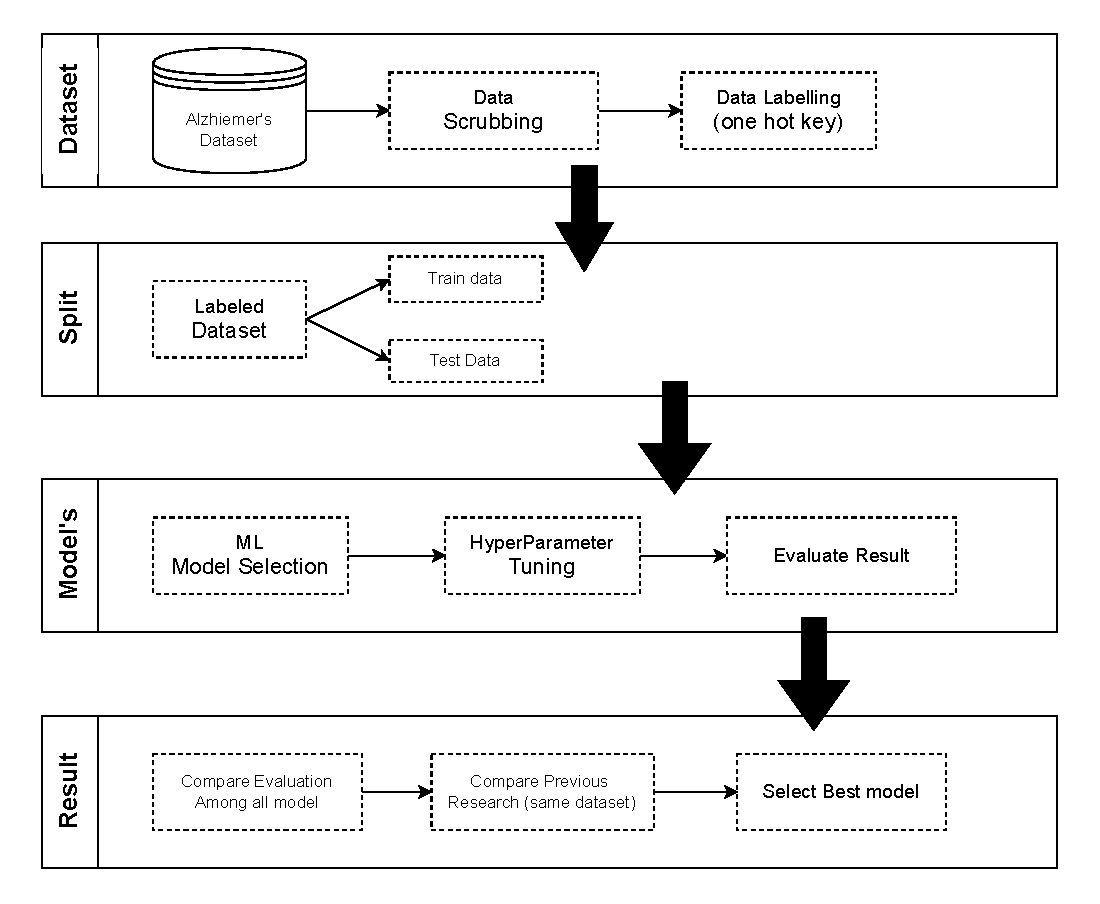
\includegraphics[width=\linewidth]{Fig-00.pdf}
    \caption{}
    \label{fig:00}
\end{figure}
\FloatBarrier

\subsection{Data Collection }
For this research, Alzheimer dataset was used from an existing paper \textit{IMPROVING MEDICAL DIAGNOSIS WITH a HYBRID BALANCING TECHNIQUE}\cite{ref2}. This dataset contains extensive health information for 2,149 patients which licensed by \textit{ATTRIBUTION 4.0 INTERNATIONAL} \cite{ref3}. This data set has 35 features and 2149 rows. It includes details fig-\ref{fig:dbdetails} like age, gender, ethnicity, and education level, along with health habits such as BMI, smoking, alcohol consumption, physical activity, and sleep quality. It also covers medical conditions like diabetes, hypertension, and depression, as well as family history of Alzheimer’s and issues with memory. And , it contains scores from health assessments and information about cognitive challenges. The main goal of the dataset is to explore how these factors connect to the diagnosis being studied.
\begin{figure}[ht]
    \centering
    \includegraphics[width=\linewidth]{Fig-03.pdf}
    \caption{}
    \label{fig:dbdetails}
\end{figure}
\FloatBarrier

The bar chart shows (fig -\ref{fig:dbdis})  the class distribution for the "Diagnosis" variable, where 0 represents "No" and 1 represents "Yes". It shows that the majority of the cases fall under the "No" category, besides  a smaller number  are classified as "Yes". 
\begin{figure}[ht]
    \centering
    \includegraphics[width=\linewidth]{Fig-02.pdf}
    \caption{}
    \label{fig:dbdis}
\end{figure}
\FloatBarrier

\subsection{Data Scrubbing}
Scrubbing is the technical process of refining data set to make it more workable which can  involve modifying and some times removing incomplecte, incorrectly formatted, irrelevant or duplicated data \cite{ref4}.In this data set feature Patient ID and Doctor In Charge does not provide any useful information for identify Alzheimer.For This research remove both column.After choosing variable and rows look for text-based features which can be converted into an number.
\subsection{Dataset split}
Using machine learning models, the dataset is divided into two subsets: train data and test data, with 80\% for training the model and 20\% for testing ( figure-\ref{fig:datasplit}) and avoid bias this research split data randomize and use Scikit-learn\cite{ref5} for randomize.

\textbf{Training Data }This part includes 1719 of the total data. It helps train the model to recognize patterns from the text and related mental health statuses.

\textbf{Test Data} The remaining 430 of the data is used to evaluate how well the model works.

\begin{figure}[ht]
    \centering
    \includegraphics[width=\linewidth]{Fig-01.pdf}
    \caption{}
    \label{fig:datasplit}
\end{figure}
\FloatBarrier

\subsection{Hyperparameter Tuning}
Hyperparameter tuning is essential for optimizing the performance and generalization of machine
learning (ML) models\cite{ref6}. This table\ref{tab:Hyperparameters} presents the hyperparameter configurations employed in various machine learning models for this research. The Logistic Regression model utilizes a regularization parameter C=10. For the Random Forest algorithm, the number of estimators is set to 200, with no limitation on the maximum depth of the trees. The AdaBoost model employs 50 estimators. While the Gradient Boosting and XGBoost models were not used in this study, the Support Vector Machine (SVM) is configured with a linear kernel and a regularization parameter C=1. The K-Nearest Neighbors (KNN) model is defined with n\_neighbors=7, and the Decision Tree model operates with a maximum depth of 5. These configurations were tailored to optimize the performance of each algorithm on the dataset.
\begin{table}[]
\centering
\caption{Hyperparameters}
\label{tab:Hyperparameters}
\begin{tabular}{|l|l|}
\hline
\multicolumn{1}{|c|}{Model} & \multicolumn{1}{c|}{Parameters}              \\ \hline
Logistic Regression         & \{'C': 10\}                                  \\ \hline
Random Forest               & \{'max\_depth': None, 'n\_estimators': 200\} \\ \hline
AdaBoost                    & \{'n\_estimators': 50\}                      \\ \hline
Gradient Boosting           & not used                                     \\ \hline
XGBoost                     & not used                                     \\ \hline
SVM                         & \{'C': 1, 'kernel': 'linear'\}               \\ \hline
KNN                         & \{'n\_neighbors': 7\}                        \\ \hline
Decision Tree               & \{'max\_depth': 5\}                          \\ \hline
\end{tabular}
\end{table}
\FloatBarrier


\subsection{Model Evaluation} 

The performance of the model can be evaluated using various metrics: accuracy\ref{eq1}, precision\ref{eq2}, recall\ref{eq3}, and F1-score\ref{eq4}, all together giving insight into the effectiveness of the model, each from a different viewpoint on the abilities of the classifier. 

Accuracy basically gives the overall correctness of the model's prediction-that is, the number of correctly classified instances divided by the total number of instances for which the model has made a prediction. Mathematically, it is represented as: 
\begin{equation}
    Accuracy =\frac{TP+TN}{TP+FP+TN+FN}
    \label{eq1}
\end{equation}
Precision depicts the capability of a model to predict actual positive instances-or, in other words, the ratio of true positives within the overall predicted positives. Precision is mathematically represented as: 
\begin{equation}
    Precision =\frac{TP}{TP+FP}
    \label{eq3}
\end{equation}
Recall, or true positive rate, gives the model's ability to capture all actual positives. It is calculated by finding the ratio of true positives to the sum of true positives and false negatives:  
\begin{equation}
    Recall =\frac{TP}{TP+FN}
    \label{eq2}
\end{equation}
The F1-score is the harmonic average of precision and recall. This gives a fair measure when both precision and recall are important. It is defined as follows:  
\begin{equation}
    F1 Score =\frac{2(Recall \times Precision)}{Recall+Precision}
    \label{eq4}
\end{equation}
Where: 
\begin{itemize}
    \item TP is True Positive,
    \item TN is True Negative,
    \item FP is False Positive,
    \item FN is False Negative.
\end{itemize}
True positive(TP) happens when the model correctly identifies requirement as Functional.
On the other hand , False Positive occurs when the model predict wrong. 
These metrics provide a granular analysis of model performance for the classification task, thereby enabling a deep understanding of strengths and weaknesses.

\section{Result and discussion}
Table -\ref{tab:classifiation} classification evaluation of various machine learning techniques(including KNN, Decision Trees, Naive Bayes, SVM) on Alzheimer’s Disease dataset using Precision,Recall and F1 Score. Note here that 1 indicates next stage with Alzheimer's Disease and 0 indicates next stage without it.
The top performers Gradient Boosting and XGBoost increase their weighted F1 Scores to 0.96 and 0.95, respectively, as a result of the most favorable mode of both classes. Other models like Random Forest and Decision Tree do well, too, getting scores of 0.92 and 0.93, respectively, while Logistic Regression and SVM underperform significantly at 0.82. In contrast, Naive Bayes is almost as good as KNN in a classification problem, while the model KNN struggles to determine correctly a class-1 outcome.
Ensemble algorithms such as Gradient Boosting and XGBoost are strikingly accurate, which underlines their suitability for intricate medical data. 
% Please add the following required packages to your document preamble:
% \usepackage{multirow}
\begin{table}[H]
\centering
\caption{Model Classification Table}
\label{tab:classification}
\resizebox{\columnwidth}{!}{%
\begin{tabular}{|c|c|c|c|c|c|c|}
\hline
\multirow{}{}{\textit{\textbf{Model}}}      & \multirow{}{}{\textit{\textbf{Class}}} & \multirow{}{}{\textit{\textbf{Precision}}} & \multirow{}{}{\textit{\textbf{Recall}}} & \multirow{}{}{\textit{\textbf{F1-Score}}} & \multicolumn{2}{c|}{\textit{\textbf{Average(F1-Score)}}}                  \\ \cline{6-7} 
                                              &                                          &                                              &                                           &                                             & \multicolumn{1}{c|}{\textit{\textbf{weighted}}} & \textit{\textbf{macro}} \\ \hline
\multirow{}{}{\textit{Logistic Regression}} & 0                                        & 0.85                                         & 0.89                                      & 0.87                                        & \multirow{}{}{0.82}                           & \multirow{}{}{0.81}   \\
                                              & 1                                        & 0.78                                         & 0.71                                      & 0.74                                        &                                                 &                         \\ \hline
\multirow{}{}{\textit{Random Forest}}       & 0                                        & 0.92                                         & 0.98                                      & 0.95                                        & \multirow{}{}{0.92}                           & \multirow{}{}{0.93}   \\
                                              & 1                                        & 0.96                                         & 0.84                                      & 0.90                                        &                                                 &                         \\ \hline
\multirow{}{}{\textit{AdaBoost}}            & 0                                        & 0.92                                         & 0.95                                      & 0.94                                        & \multirow{}{}{0.92}                           & \multirow{}{}{0.91}   \\
                                              & 1                                        & 0.91                                         & 0.85                                      & 0.88                                        &                                                 &                         \\ \hline
\multirow{}{}{\textit{Gradient Boost}}      & 0                                        & 0.96                                         & 0.97                                      & 0.97                                        & \multirow{}{}{0.96}                           & \multirow{}{}{0.95}   \\
                                              & 1                                        & 0.95                                         & 0.92                                      & 0.94                                        &                                                 &                         \\ \hline
\multirow{}{}{\textit{XGBoost}}             & 0                                        & 0.94                                         & 0.98                                      & 0.96                                        & \multirow{}{}{0.95}                           & \multirow{}{}{0.94}   \\
                                              & 1                                        & 0.96                                         & 0.90                                      & 0.93                                        &                                                 &                         \\ \hline
\multirow{}{}{\textit{Naive Bayes}}         & 0                                        & 0.77                                         & 0.74                                      & 0.76                                        & \multirow{}{}{0.69}                           & \multirow{}{}{0.67}   \\
                                              & 1                                        & 0.56                                         & 0.60                                      & 0.58                                        &                                                 &                         \\ \hline
\multirow{}{}{\textit{SVM}}                 & 0                                        & 0.84                                         & 0.88                                      & 0.86                                        & \multirow{}{}{0.82}                           & \multirow{}{}{0.80}   \\
                                              & 1                                        & 0.77                                         & 0.71                                      & 0.74                                        &                                                 &                         \\ \hline
\multirow{}{}{\textit{KNN}}                 & 0                                        & 0.63                                         & 0.74                                      & 0.68                                        & \multirow{}{}{0.55}                           & \multirow{}{}{0.48}   \\
                                              & 1                                        & 0.32                                         & 0.22                                      & 0.26                                        &                                                 &                         \\ \hline
\multirow{}{}{\textit{Decision Tree}}       & 0                                        & 0.93                                         & 0.96                                      & 0.94                                        & \multirow{}{}{0.93}                           & \multirow{}{}{0.92}   \\
                                              & 1                                        & 0.92                                         & 0.87                                      & 0.90                                        &                                                 &                         \\ \hline
\end{tabular}
}
\end{table}
\FloatBarrier




As shown in table-\ref{tab:evaluation} and graphically represent fig-\ref{fig:evaluation}, the obtainment of evaluation metric values for different Machine Learning approaches in prediction techniques for AD classification on the dataset. With the highest scores (0.95 across all metrics), Gradient Boosting proved to be the most robust, striking a good balance between precision and recall.Closer behind were XGBoost and Random Forest with similar metrics and showing that ensemble methods work better.On the other hand, Naive Bayes (0.69) could not handle complex feature interaction well, and KNN (0.55) had the least ability to model this dataset. This study highlights the effectiveness of ensemble methods, such as Gradient Boosting, XGBoost, and Random Forest, for classification tasks in Alzheimer’s Disease, providing a useful reference for researchers working on predictive modeling in medicine.

Over all this research find that Gradient boosting earn height performance among all model.
\begin{table}[]
\centering
\caption{Model Evaluation Metrics}
\label{tab:evaluation}
\begin{tabular}{|l|ccc|c|}
\hline
\multicolumn{1}{|c|}{\textit{\textbf{Model}}} & \textit{\textbf{Precision}} & \textit{\textbf{Recall}} & \textit{\textbf{F1-Score}} & \textit{\textbf{Accuracy}} \\ \hline
\textit{\textbf{Logistic Regression}}         & 0.82                        & 0.82                     & 0.82                       & 0.82                       \\ \hline
\textit{\textbf{Random Forest}}               & 0.93                        & 0.93                     & 0.93                       & 0.93                       \\ \hline
\textit{\textbf{AdaBoost}}                    & 0.91                        & 0.91                     & 0.91                       & 0.91                       \\ \hline
\textit{\textbf{Gradient Boost}}              & 0.95                        & 0.95                     & 0.95                       & 0.95                       \\ \hline
\textit{\textbf{XGBoost}}                     & 0.94                        & 0.94                     & 0.94                       & 0.94                       \\ \hline
\textit{\textbf{Naive Bayes}}                 & 0.69                        & 0.69                     & 0.69                       & 0.69                       \\ \hline
\textit{\textbf{SVM}}                         & 0.81                        & 0.82                     & 0.81                       & 0.82                       \\ \hline
\textit{\textbf{KNN}}                         & 0.51                        & 0.55                     & 0.53                       & 0.55                       \\ \hline
\textit{\textbf{Decision Tree}}               & 0.92                        & 0.92                     & 0.92                       & 0.92                       \\ \hline
\end{tabular}
\end{table}
\FloatBarrier

\begin{figure}[ht]
    \centering
    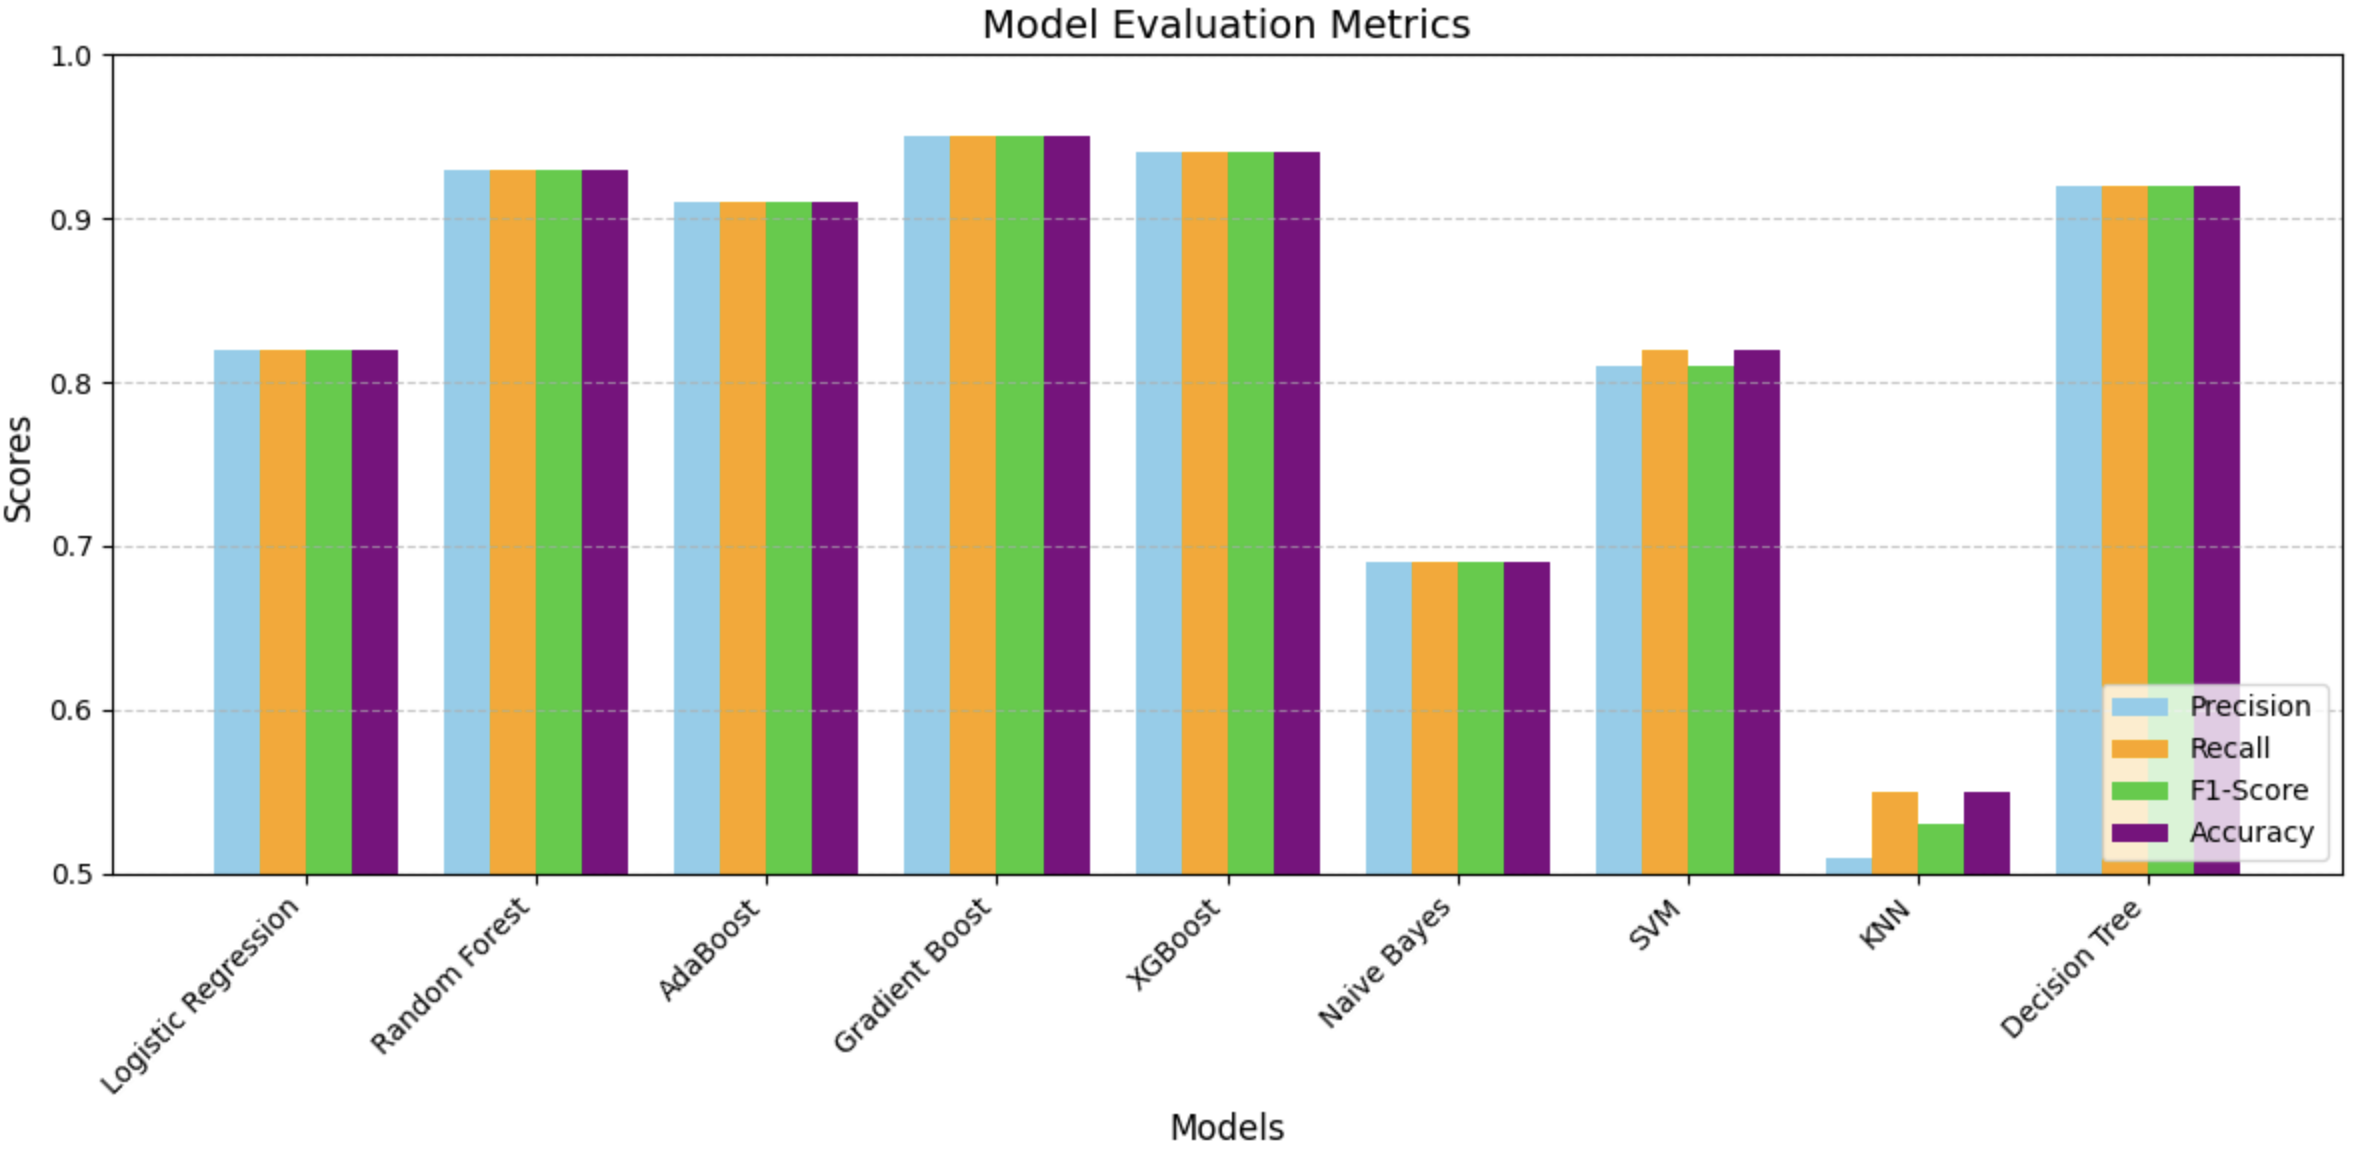
\includegraphics[width=\linewidth]{Fig-05.png}
    \caption{}
    \label{fig:evaluation}
\end{figure}
\FloatBarrier

\subsection{Previous Study Result}
Table-\ref{tab:previousres} shows the performance from previous studies on similar tasks and data sets (Airlangga,2024)\cite{com1} used CNN and achieved 88.65\% accuracy. Buribayev et al. (2024b)\cite{com2} finding slightly higher accuracy(81.95\%) with LM model approach.


\begin{table}[]
\centering
\caption{Model Accuracy Comparison with Citations}
\label{tab:previousres}
\begin{tabular}{lcc}
\hline
\textbf{Citation}                                  & \textbf{Model} & \textbf{Accuracy (\%)} \\ \hline
(Airlangga, 2024)\cite{com1}        & CNN            & 88.65                  \\
Buribayev et al. (2024b)\cite{com2} & LR             & 84.0                   \\ \hline
\end{tabular}
\end{table}
\FloatBarrier

According to previous paper, this research also achieve higher accuracy using \textbf{Gradient Boost} which is \textbf{95.0\%}.

Fig-\ref{fig:confussion} indicates confusion matrix for Gradient Boost. The confusion matrix is the table that summarizes how successful the classification model is at prediction examples belonging to various classes.\cite{ref4}.In this figure x axis shows predicted label and other axis Y shows actual label. In this case 0 indecates without Alzheimer's and 1 indicates effected with Alzheimer. There are in total 278 examples that actually without Alzheimer and correctly classified 271 as True positive(TP) and in incorrectly classified 6 as False Negative (FN). On the other hand 1 class (with Alzheimer) correctly identify 141 as true negative(TN) and incorrectly identify 12 samples as False Negative(FN) where total samples were 153.

\begin{figure}[ht]
    \centering
    \includegraphics[width=\linewidth]{Fig-04.pdf}
    \caption{}
    \label{fig:confussion}
\end{figure}
\FloatBarrier


\textbf{Cohen's Kappa Score Calculation:}Cohen’s kappa statistic is a widely used measure of agreement between two raters, particularly in assessing interrater reliability \cite{ref7}. This statistical measure ranges from (ϑ1) to (+1) in most correlation analyzes. The calculation of Cohen’s kappa coefficient in this study was based on the confusion matrix (Fig. \ref{fig:confussion}). The formula for Cohen’s kappa coefficient is as follows \cite{ref8}:

\[
\kappa = \frac{P_o - P_e}{1 - P_e}
\]

where $P_o$ is the observed agreement and $P_e$ is the expected agreement.

\textbf{Observed Agreement ($P_o$)}
\[
P_o = \frac{\text{Sum of Diagonal Elements}}{\text{Total Number of Instances}}
\]
\[
P_o = \frac{271 + 141}{430}
\]
\[
P_o \approx 0.96
\]

\textbf{Expected Agreement ($P_e$)}
\[
P_e = \frac{\sum (\text{Row Total} \times \text{Column Total})}{(\text{Total Number of Instances})^2}
\]
\[
P_e = \frac{(271 + 12) \times (271 + 6) + (141 + 12) \times (141 + 6)}{(430)^2}
\]
\[
P_e = \frac{(283 \times 277) + (153\times 147)}{430^2}
\]
\[
P_e = 0.545
\]

\textbf{Evaluating Cohen's Kappa Score}
\[
\kappa = \frac{0.96 - 0.545}{1 - 0.545}
\]
\[
\kappa = \frac{0.415}{0.455}
\]
\[
\kappa \approx 0.912
\]
According to Datatab \cite{ref1} Cohen’s Kappa score of 0.9974 indicates outstanding performance.


This graph fig-\ref{fig:10fold} indicates the 10-Fold Cross-Validation Accuracy for the Gradient Boosting model. Most folds shows high accuracy (~1.0) and perform well , But there is a shape drop on 10th folds. The red dash line shows the average accuracy across all folds, serving as a baseline.
\begin{figure}[ht]
    \centering
    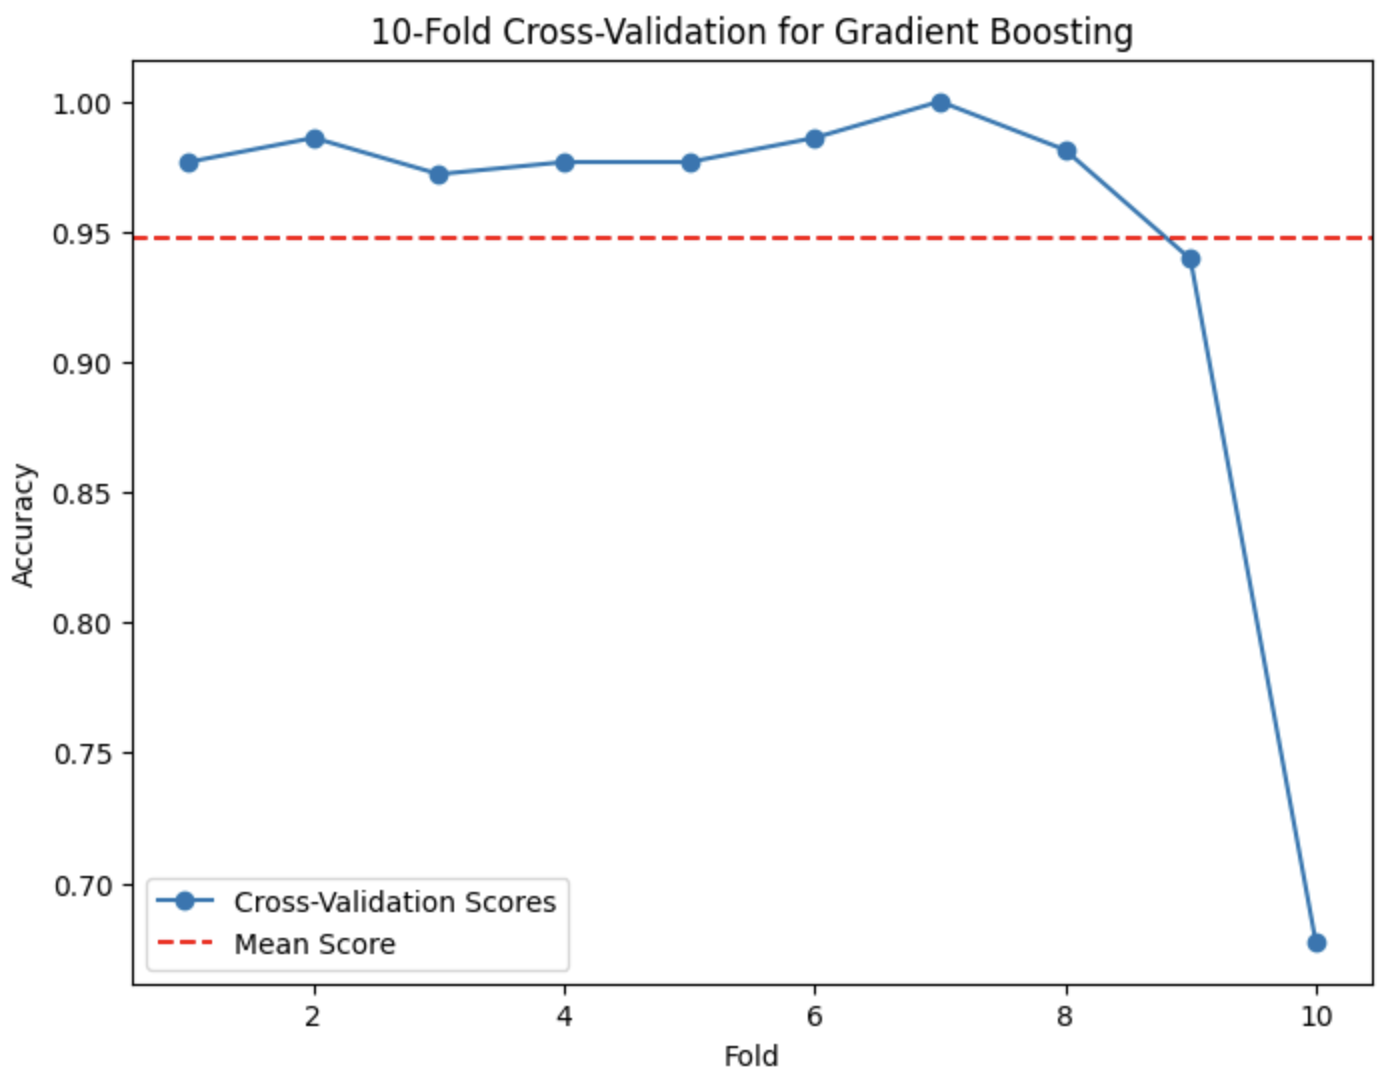
\includegraphics[width=\linewidth]{Fig-06.png}
    \caption{}
    \label{fig:10fold}
\end{figure}
\FloatBarrier

Precision-Recall (PR) curve(fig-\ref{fig:08} shows that the Gradient Boosting classifier is both an excellent precision scorer and really good at handling imbalanced data. The model starts with almost perfect precision indicating its ability to correctly identify most of the positive samples at the cost of few false positives. While increasing recall, precision slowly begins to fall until many false-positives have been accepted too for finding all but a few positive samples. It thus appears perfectly calibrated when being used in a context where precision-recall trade-off is needed or for dealing with imbalanced-class problems because it gives high precision for every level of recall.

\begin{figure}[ht]
    \centering
    \includegraphics[width=\linewidth]{Fig-08.pdf}
    \caption{}
    \label{fig:08}
\end{figure}
\FloatBarrier


The learning curve \ref{fig:09} for the Gradient Boosting classifier demonstrates the connection between the performance of the model and the training dataset size, and thus gives us a glimpse of its generalization capabilities. The training score exhibits a constant high value close to 1.0 among all training sizes, which means that the model is fitting the training data well. In contrast, the cross-validation score starts low and grows with increased training data, finally interacting with the training score. It is a reality that the model will improve with the addition of more training samples because it will have better results, lower variance, and better generalization to new data. The shrinking difference between the training and cross-validation scores as the data grows, shows that it gets less overfitting. The areas that are shaded signal to the variability of the scores, with the cross-validation variance which slowly fades away, thus strengthening the model at bigger training sizes. This study shows that Gradient Boosting is an efficient method with enough data and it projects the possibility for accurate predictions in real-life applications.

\begin{figure}[ht]
    \centering
    \includegraphics[width=\linewidth]{Fig-09.pdf}
    \caption{}
    \label{fig:09}
\end{figure}
\FloatBarrier

The correlation heatmap (fig-\ref{fig:heatmap}) is the visual representation of how strongly pairwise relationships are closely related. This indication exemplifies the linear correlation between those variables, which can have different values ranging from -1 to +1 or zero between them. Indeed, the diagonal itself contains all such diagonal elements equal to 1, since every variable must necessarily be perfectly correlated with itself. The effective feature correlations (such as > 0.7 or < -0.7) usually reiterate redundancy or multicollinearity in your variables affecting predictive models and may require you to remove one of those variables for easier analysis. Features, on the other hand, that have very little correlation with the others may hold important information so you would want to look at it closely.

These features with strong correlations toward the target variable ('Diagnosis') are the most significant and influencing features for modeling, while weakly correlated features would have to be analyzed in the future relative to their meaning. Enhance analysis with feature selection techniques and/or dimensionality reduction methods such as PCA against redundancy in highly correlated features. Correlation findings may lead to proper variable prioritization in regression or classification assignments, inspire future exploration of significant associations to unearth possible causal links, etc.

\begin{figure}[ht]
    \centering
    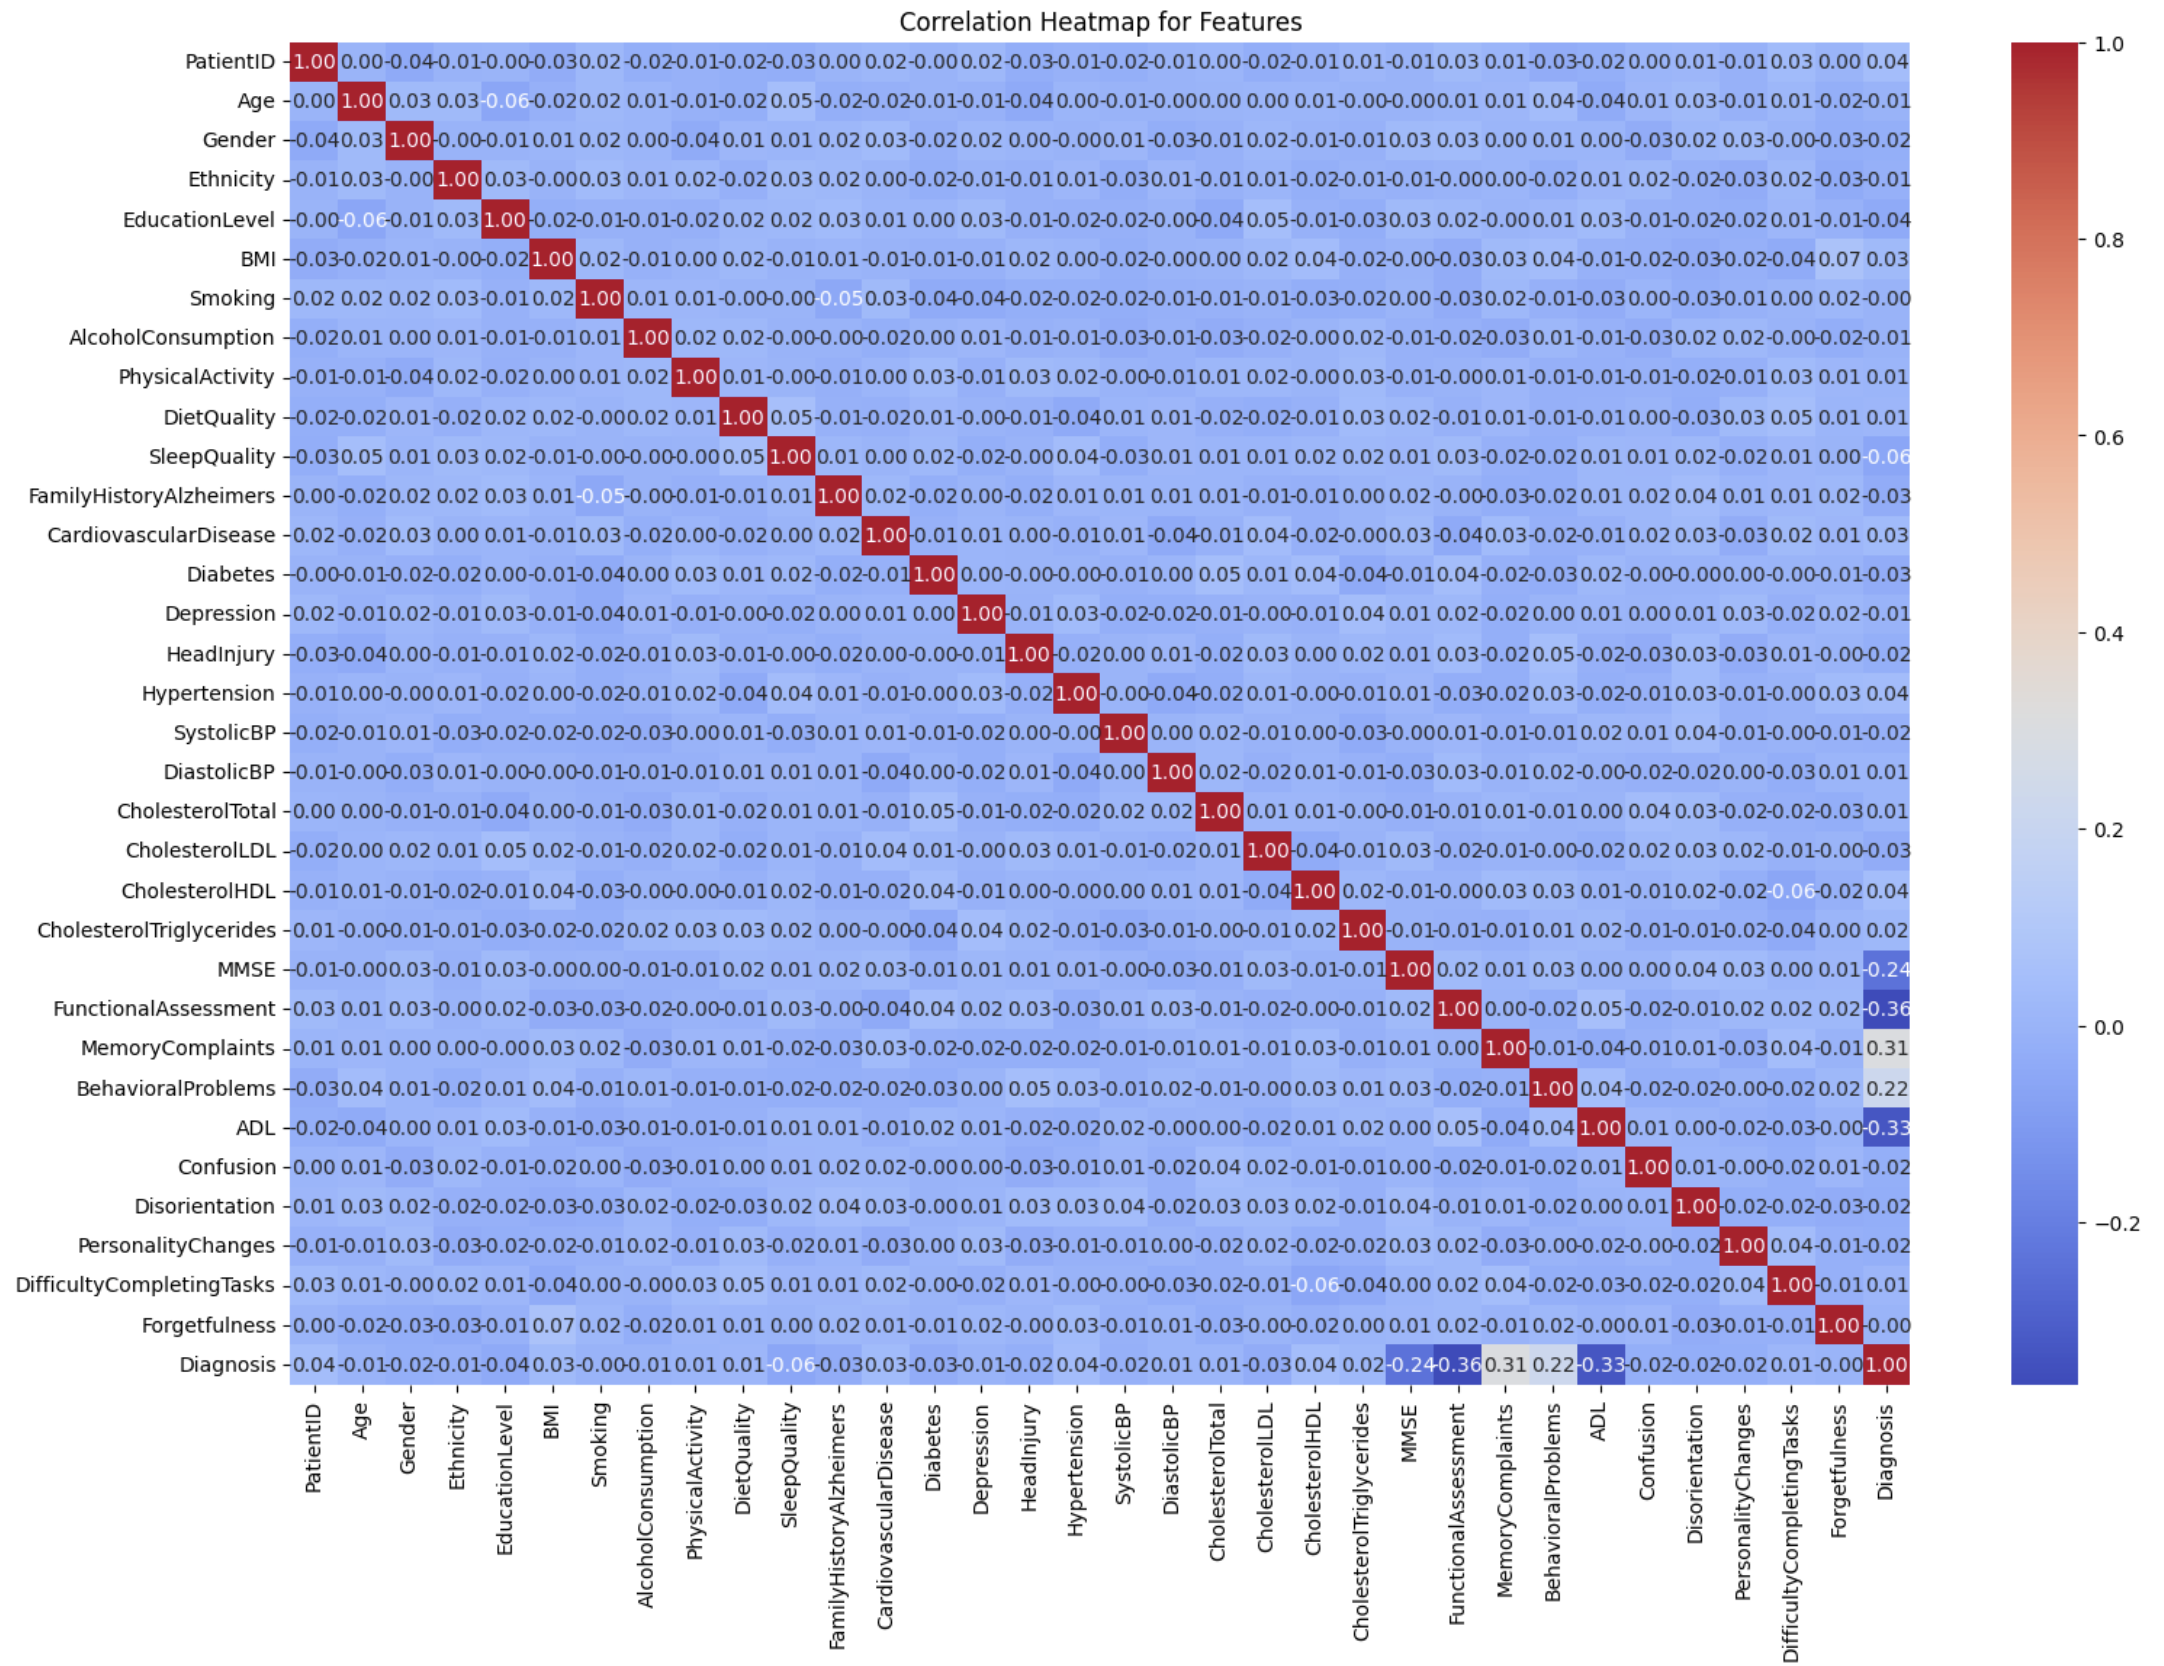
\includegraphics[width=\linewidth]{Fig-07.png}
    \caption{}
    \label{fig:heatmap}
\end{figure}
\FloatBarrier

The SHAP summary plot figure-\ref{fig:10} shows a clear view of the features that hold the most significance for the model and how they influence predictions. The y-axis organizes the features based on their importance, while the x-axis shows SHAP values, reflecting each feature's contribution to the model's results.A positive SHAP value signifies that the feature boosts the prediction, whereas a negative value indicates a reduction in the prediction. Each dot on the plot represents a data point, with colors ranging from blue to red to indicate whether the feature value is low (blue) or high (red). However, the plot demonstrates that predictions differ greatly with enough variability in the SHAP values of FunctionalAssessment and ADL, which were evident within the plot. For example, if FunctionalAssessment is greater than a certain threshold value then the predictions would be more. On the other hand, features like BehavioralProblems are likely to reduce the predictions of the values of the given feature. Less important attributes – EducationLevel, and Depression, also have minimal influence over the model, as their SHAP values are not significantly affected.  Closer inspection of how the model sheds light on the individual predictors eases the interpretation of feature importance and identifies the relationship between a given feature and the output. Indeed, such ideas are critical in making improvements to the model and guaranteeing the model will be properly implemented on sectors that need it.

\begin{figure}[ht]
    \centering
    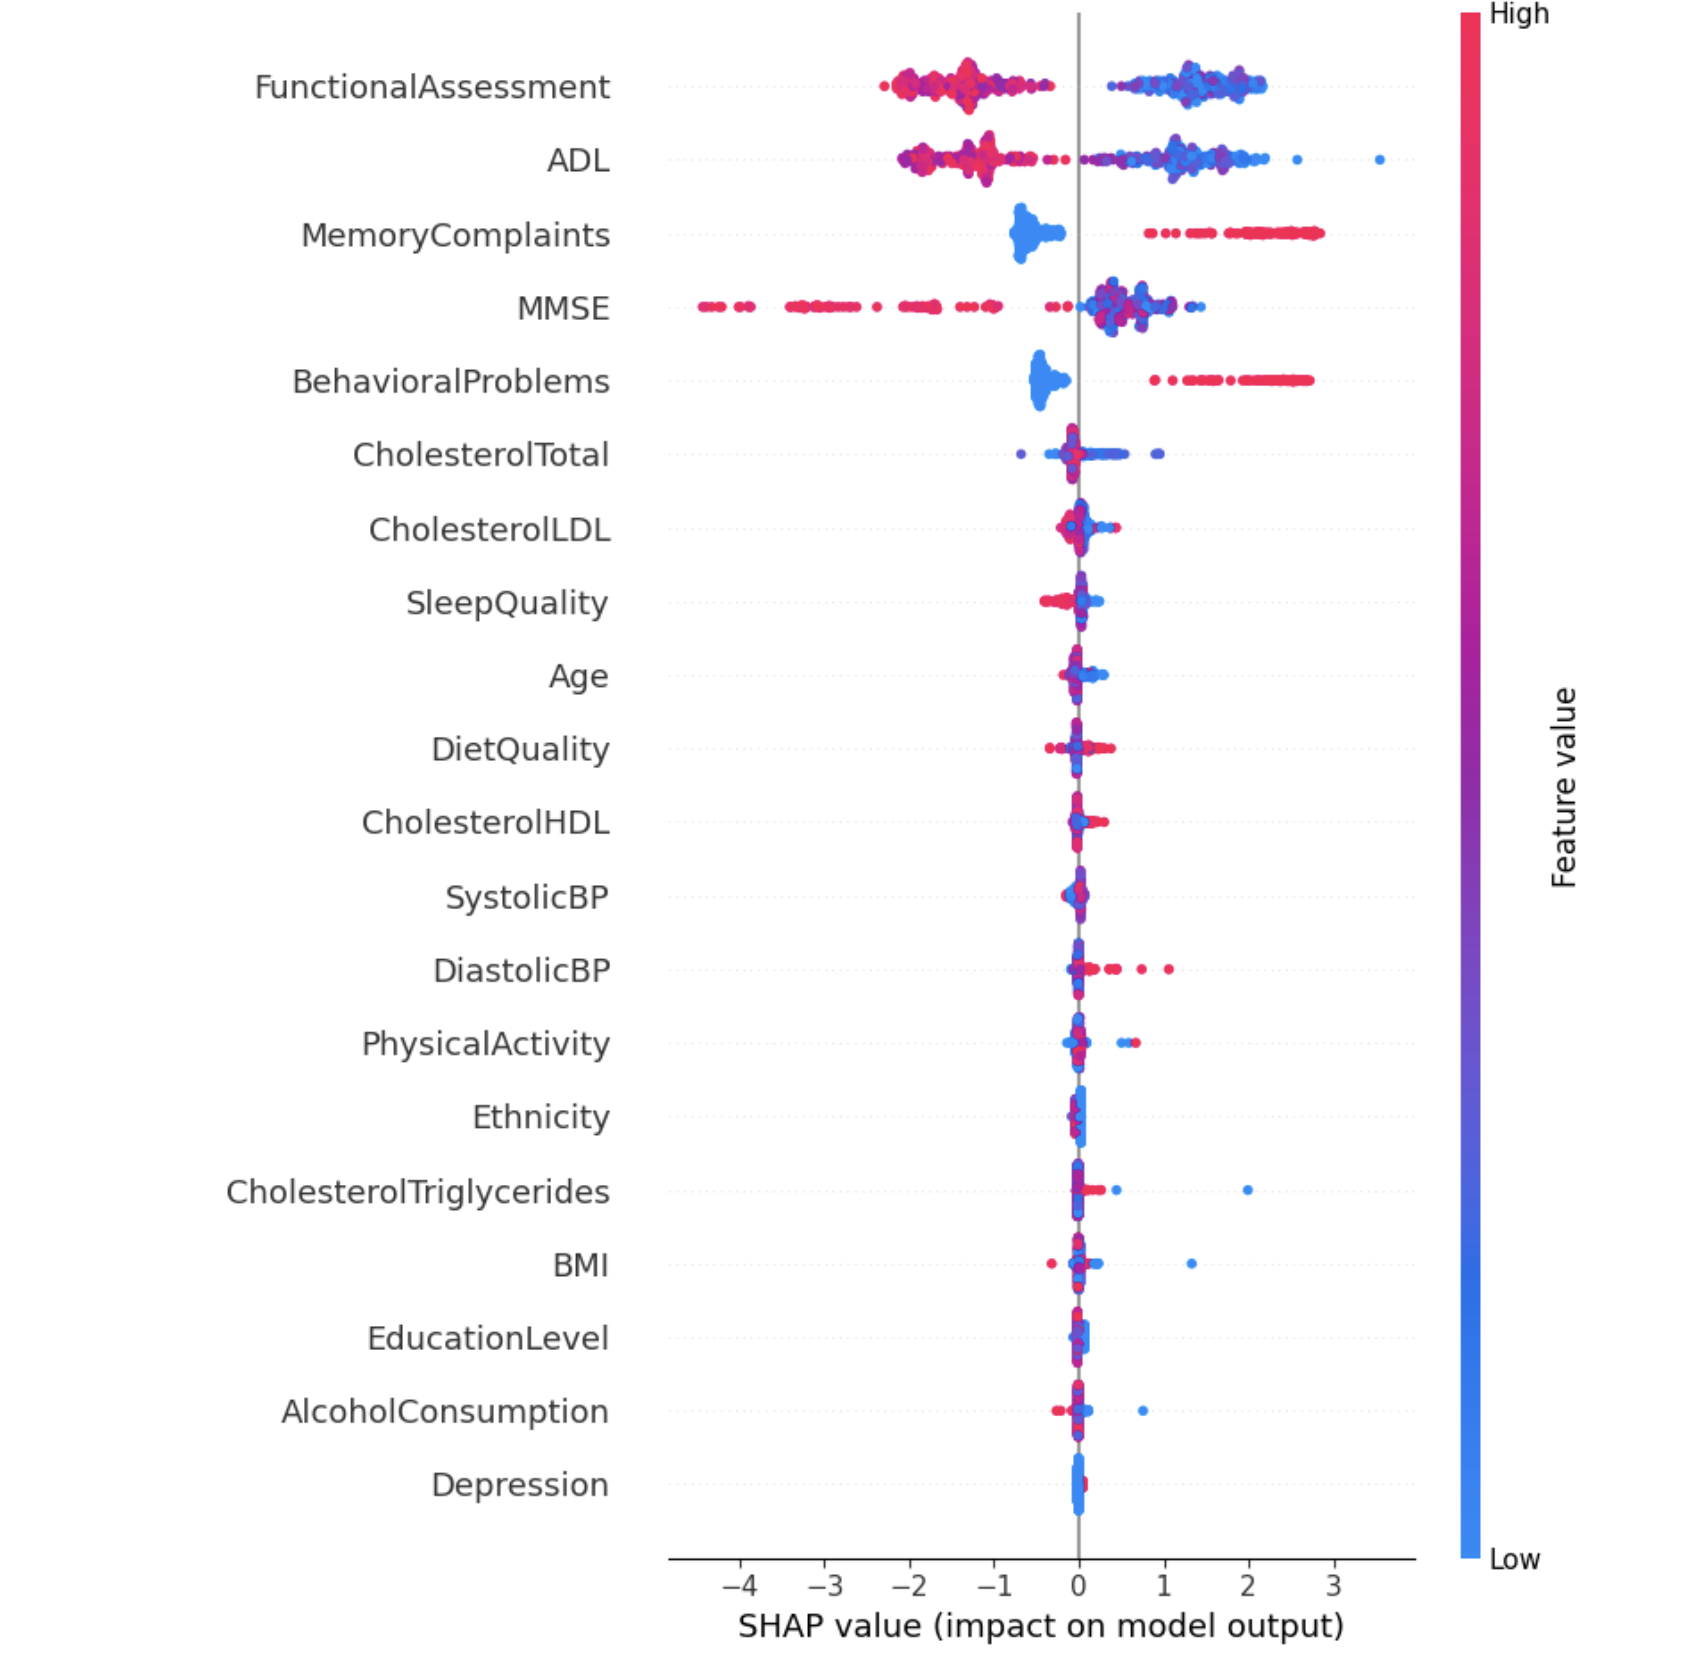
\includegraphics[width=\linewidth]{Fig-10.png}
    \caption{}
    \label{fig:10}
\end{figure}
\FloatBarrier



\section{Conclusion}

This study has shown a positive result by using the ensemble machine learning technique primarily through Gradient Boosting applied to Alzheimer's Disease diagnosis. This Gradient Boosting model achieved 95 percent accuracy, which is far better than other methods, including traditional algorithms and simpler ensemble methods. The research also elaborated on how relevant preprocessing, balanced datasets, and hyperparameter optimization are for making accurate predictions. However, model interpretability and system resource requirements remain mostly on the to-do list of the researchers. Future work will seek ways in integrating future data sources of excellent quality and quantity to diversify the dataset for research on advanced techniques in feature selection to improve model generalizability. The study will help serve as a reference point to further research as well as clinicians towards feeding some way to diagnostics that can engage the battle against Alzheimer's Disease into more accurate and scalable solutions.




%References
\begin{thebibliography}{8}
\bibitem{ref1}
T-Test, Chi-Square, ANOVA, Regression, Correlation. . . (n.d.). https://datatab.net/tutorial/cohens-kappa

\bibitem{ref2}
Buribayev, Z., Yerkos, A., Shaikalamova, S., Imanbek, R., \& Zhetpisbay, Z. (2024). IMPROVING MEDICAL DIAGNOSIS WITH a HYBRID BALANCING TECHNIQUE. Journal of Problem in Computer Science and Information Technologies, 2(3), 11–20. https://doi.org/10.26577/jpcsit2024-02i03-02

\bibitem{ref3}
Deed - Attribution 4.0 International - Creative Commons. (n.d.). https://creativecommons.org/licenses/by/4.0/

\bibitem{ref4}
Theobald, O. (2017). Machine learning for absolute beginners (Second Edition).

\bibitem{ref5}
train\_test\_split. (n.d.). Scikit-learn. https://scikit-learn.org/1.5/modules/generated/sklearn.mode\_selection.train\_test\_split.html

\bibitem{ref6}
Ilemobayo, J. A., Durodola, O., Alade, O., Awotunde, O. J., Olanrewaju, A. T., Falana, O., Ogungbire, A., Osinuga, A., Ogunbiyi, D., Ifeanyi, A., Odezuligbo, I. E., \& Edu, O. E. (2024). Hyperparameter tuning in Machine Learning: A Comprehensive review. Journal of Engineering Research and Reports, 26(6), 388–395. https://doi.org/10.9734/jerr/2024/v26i61188

\bibitem{ref7}
A. Rogeau, F. Hives, C. Bordier, H. Lahousse, V. Roca, T. Lebouvier, F. Pasquier,
D. Huglo, F. Semah, R. Lopes, A 3D convolutional neural network to classify
subjects as Alzheimer’s disease, frontotemporal dementia or healthy controls
using brain 18F-FDG PET, NeuroImage 288 (2024) 120530.

\bibitem{ref8}
M. Masud, A.M. Almars, M.B. Rokaya, H. Meshref, I. Gad, E.-S. Atlam, A novel
light-weight convolutional neural network model to predict Alzheimer’s disease
applying weighted loss function, J. Disabil. Res. 3 (4) (2024) 20240042.

\bibitem{com1}
Airlangga, G. (2024). Advancing Alzheimer’s Diagnosis: A Comparative analysis of deep learning architectures on multidimensional health data. Jurnal Informatika Ekonomi Bisnis, 810–814. https://doi.org/10.37034/infeb.v6i4.1046


\bibitem{com2}
Buribayev, Z., Yerkos, A., Shaikalamova, S., Imanbek, R., \& Zhetpisbay, Z. (2024b). IMPROVING MEDICAL DIAGNOSIS WITH a HYBRID BALANCING TECHNIQUE. Journal of Problem in Computer Science and Information Technologies, 2(3), 11–20. https://doi.org/10.26577/jpcsit2024-02i03-02


\end{thebibliography}
\bibliographystyle{spbasic}
\bibliography{Sources.bib}

\end{document}




